\documentclass[compress,red]{beamer}
\usepackage[utf8]{inputenc}
\usepackage{ucs}
\usepackage{amsmath}
\usepackage{amsfonts}
\usepackage{amssymb}
\usepackage[russian]{babel}
\usepackage{graphicx}
\usepackage{wrapfig}

\usepackage{tikz}
\usepackage{verbatim}

\usepackage{color}
\usepackage{xcolor}
\usepackage{listings}

\usepackage{caption}

\lstset{
language=ruby,
extendedchars=\true,
inputencoding=utf8x,
commentstyle=\itshape,
stringstyle=\bf,
belowcaptionskip=5pt }


\DeclareCaptionFont{white}{\color{white}}
\DeclareCaptionFormat{listing}{\colorbox{gray}{\parbox{\textwidth}{#1#2#3}}}
\captionsetup[lstlisting]{format=listing,labelfont=white,textfont=white}

\usetikzlibrary{calc,trees,positioning,arrows,chains,shapes.geometric,%
    decorations.pathreplacing,decorations.pathmorphing,shapes,%
    matrix,shapes.symbols}

\tikzset{
>=stealth',
  punktchain/.style={
    rectangle, 
    rounded corners, 
    % fill=black!10,
    draw=black, very thick,
    text width=10em, 
    minimum height=3em, 
    text centered, 
    on chain},
  line/.style={draw, thick, <-},
  element/.style={
    tape,
    top color=white,
    bottom color=blue!50!black!60!,
    minimum width=8em,
    draw=blue!40!black!90, very thick,
    text width=10em, 
    minimum height=1.5em, 
    text centered, 
    on chain},
  every join/.style={->, thick,shorten <=1pt},
  decoration={brace},
  tuborg/.style={decorate},
  tubnode/.style={midway, right=2pt},
}

\mode<presentation>

\usetheme{Warsaw}

\definecolor{Red}{rgb}{1,0,0}
\definecolor{Blue}{rgb}{0,0,1}
\definecolor{Green}{rgb}{0,1,0}
\definecolor{magenta}{rgb}{1,0,.6}
\definecolor{lightblue}{rgb}{0,.5,1}
\definecolor{lightpurple}{rgb}{.6,.4,1}
\definecolor{gold}{rgb}{.6,.5,0}
\definecolor{orange}{rgb}{1,0.4,0}
\definecolor{hotpink}{rgb}{1,0,0.5}
\definecolor{newcolor2}{rgb}{.5,.3,.5}
\definecolor{newcolor}{rgb}{0,.3,1}
\definecolor{newcolor3}{rgb}{1,0,.35}
\definecolor{darkgreen1}{rgb}{0, .35, 0}
\definecolor{darkgreen}{rgb}{0, .6, 0}
\definecolor{darkred}{rgb}{.75,0,0}

\xdefinecolor{olive}{cmyk}{0.64,0,0.95,0.4}
\xdefinecolor{purpleish}{cmyk}{0.75,0.75,0,0}

\useoutertheme[subsection=false]{smoothbars}

\title{Электронные таблицы}

%\usecolortheme{dolphin}


\begin{document}
%%титульная страница
\maketitle
%% основные моменты

\section{Электронные таблицы}

\subsection{Электронные таблицы}
\begin{frame}[fragile]
  \frametitle{Электронные таблицы}
  \begin{itemize}
    \item Часто на практике мы имеем дело с данными, представимыми в табличном виде.
    \item Примеры: оценки в школе, прайс-лист на стоимость товаров, личный бюджет и пр.
    \item Для работы с таблицами существуют специальные программы, называемые \emph{табличными процессорами}:
      \begin{enumerate}
          \item Microsoft Excel (Windows)
          \item OpenOffice Calc (Linux)
          \item Numbers (OS X)
          \item Google Drive (Web)
      \end{enumerate}
  \end{itemize}
\end{frame}

\subsection{Google Drive создание}
\begin{frame}[fragile]
  \frametitle{Google Drive-таблицы}
  \centerline{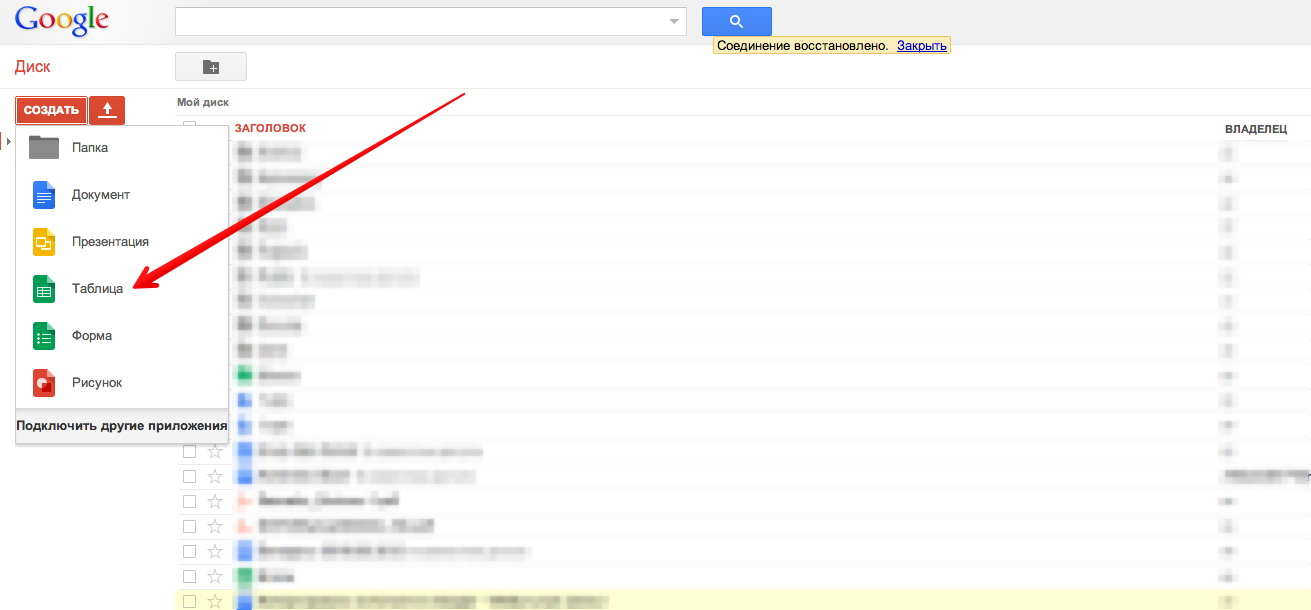
\includegraphics[width=0.9\textwidth]{images/01.png}}
  \centerline{\Large{http://drive.google.com}}
\end{frame}

\subsection{Строки и столбцы}
\begin{frame}[fragile]
  \frametitle{Строки и столбцы}
  \begin{itemize}
    \item В электронной таблице имеются:
        \begin{enumerate}
            \item \emph{Столбцы} (обозначаются латинскими буквами по алфавиту),
            \item \emph{Строки} (обозначаются последовательными натуральными числами).
        \end{enumerate}
    \item \emph{Ячейка} --- элемент электронной таблицы. У ячейки есть столбец и строка. Обозначается ячейка по их номерам: \textbf{B3, A1, F21}.
    \item Схема определения --- как в морском бое.
  \end{itemize}
\end{frame}

\subsection{Чистая таблица}
\begin{frame}[fragile]
  \frametitle{Пример электронной таблицы}
  \centerline{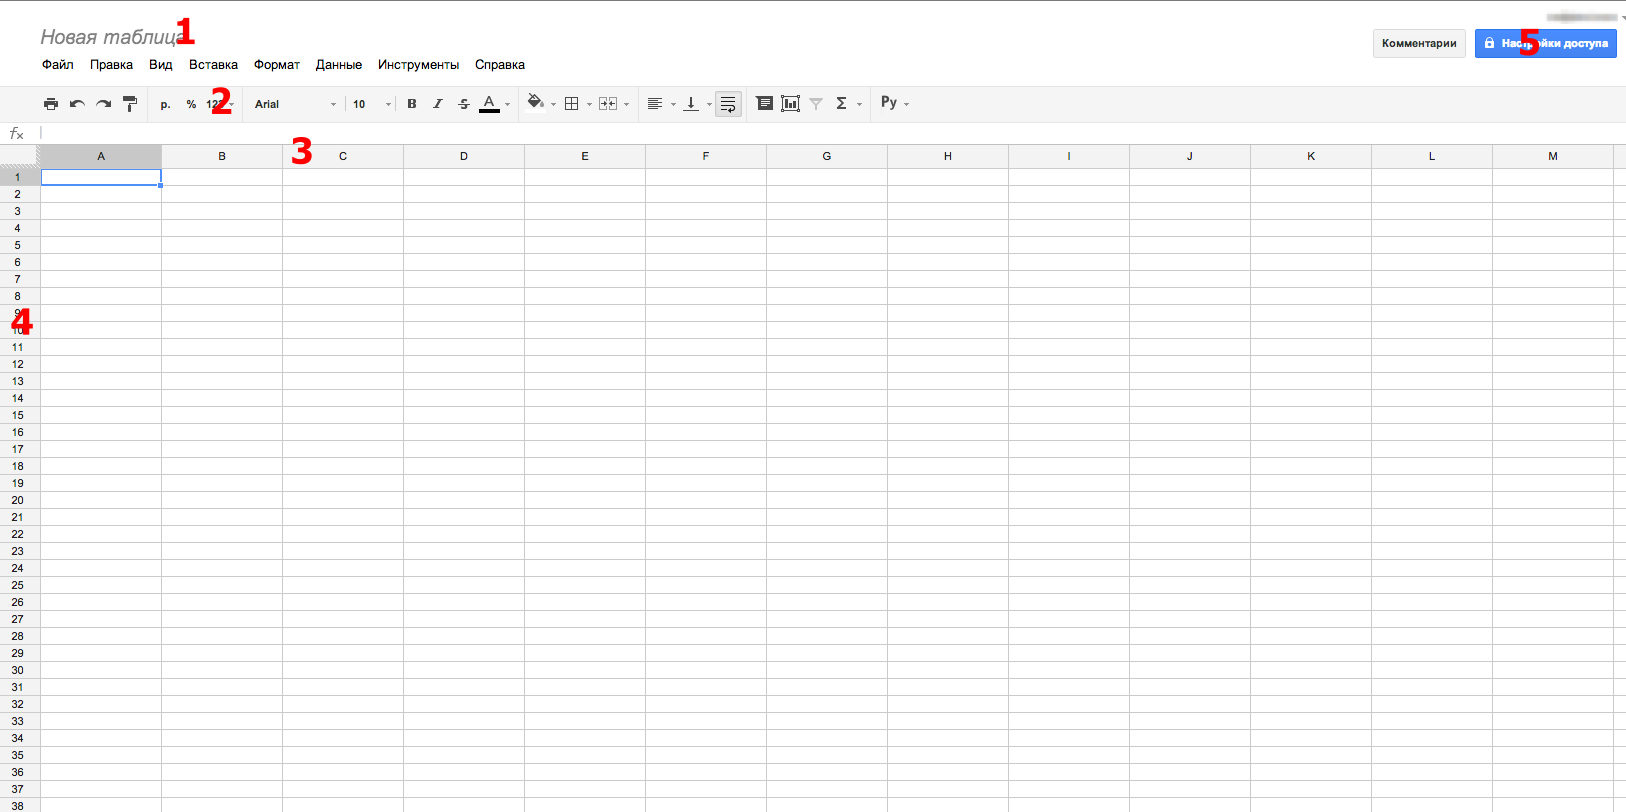
\includegraphics[width=0.9\textwidth]{images/02.png}}
\end{frame}

\subsection{Тренировка 1}
\begin{frame}[fragile]
  \frametitle{Тренировка: номера ячеек}
  \centerline{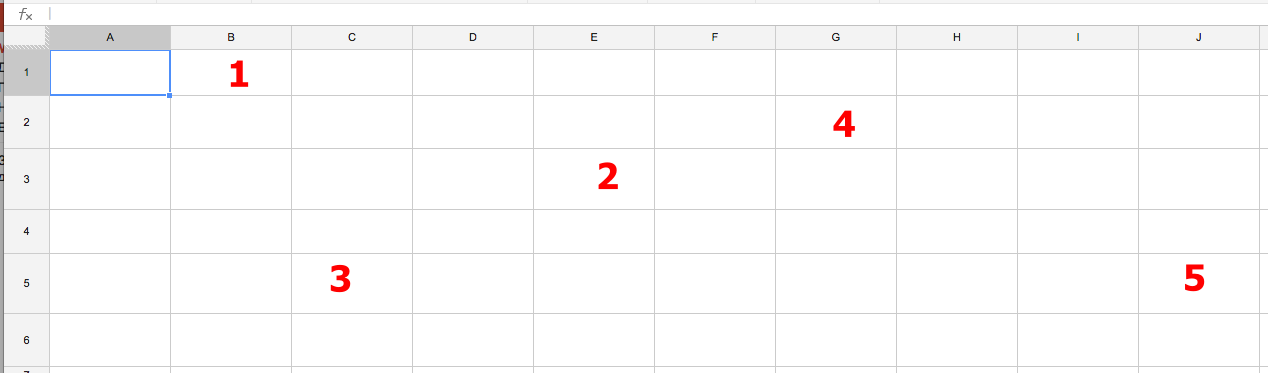
\includegraphics[width=0.9\textwidth]{images/03.png}}
  \begin{itemize}[<+->]
      \item Ячейки:
      \begin{enumerate}[<+->]
          \item B1
          \item E3
          \item C5
          \item G2
          \item J5
      \end{enumerate}
  \end{itemize}
\end{frame}

\subsection{Добавление/удаление строки}
\begin{frame}[fragile]
  \frametitle{Добавление и удаление строки}
  \centerline{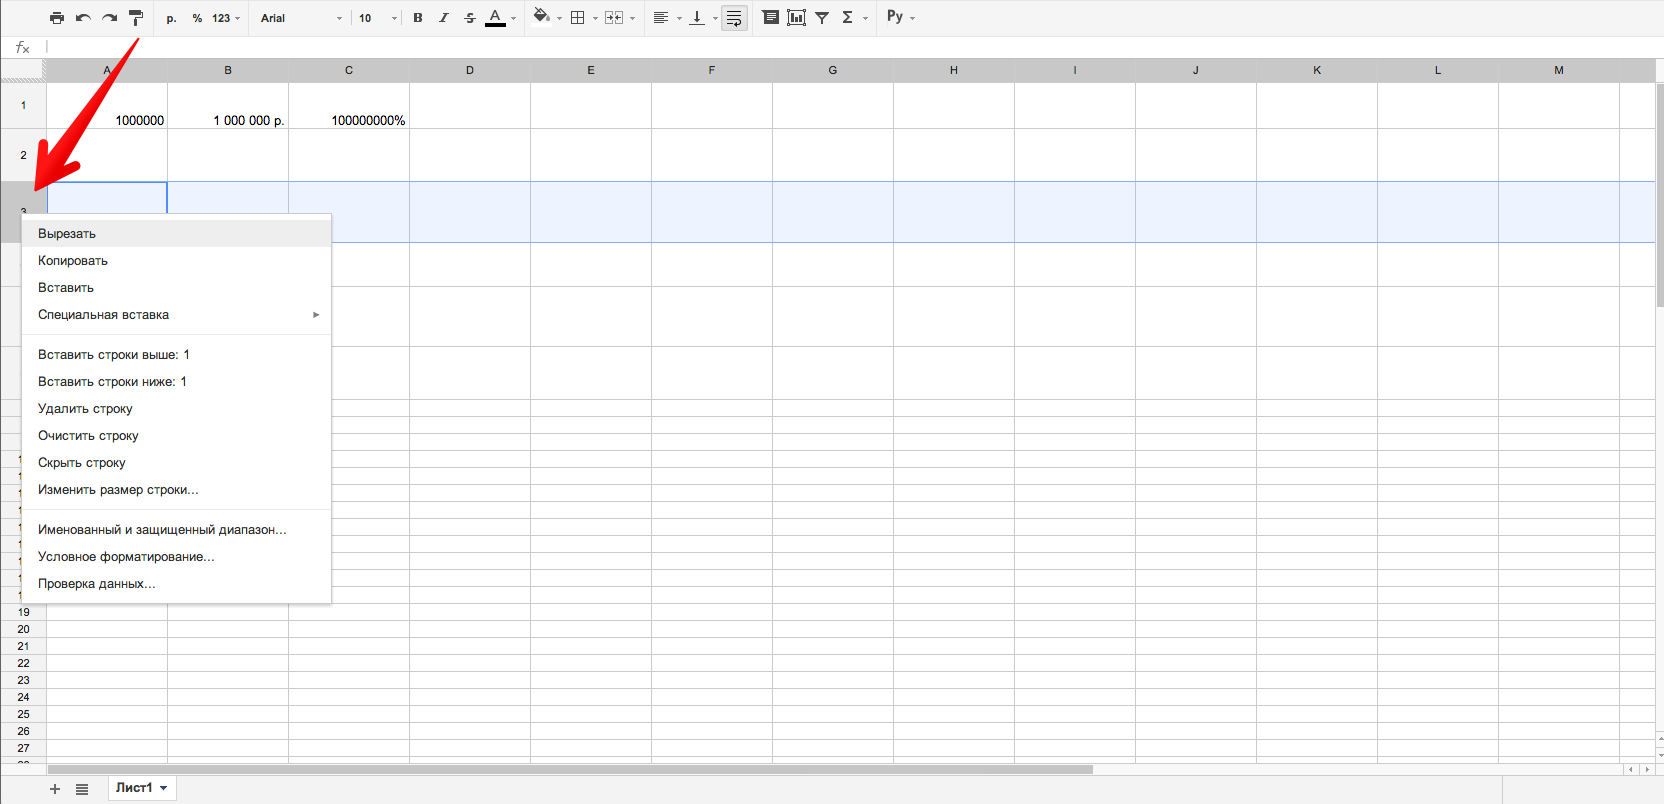
\includegraphics[width=1.0\textwidth]{images/05.png}}
  \begin{itemize}
      \item Для добавления и/или удаления строки нажимаем на название строки левой кнопкой мыши, затем правой.
      \item В выпадающем меню выбираем соответствующий пункт.
  \end{itemize}
\end{frame}

\section{Типы данных}
\subsection{Типы данных}
\begin{frame}[fragile]
  \frametitle{Типы данных}
  \begin{itemize}
    \item Ячейки могут работать с:
      \begin{enumerate}
          \item числами (целое, вещественное, валюта, процент и пр.),
          \item строки и текст,
          \item даты,
          \item \textbf{формулы}. 
      \end{enumerate}
  \end{itemize}
\end{frame}

\subsection{Скриншот типов}
\begin{frame}[fragile]
  \frametitle{Типы данных}
  \centerline{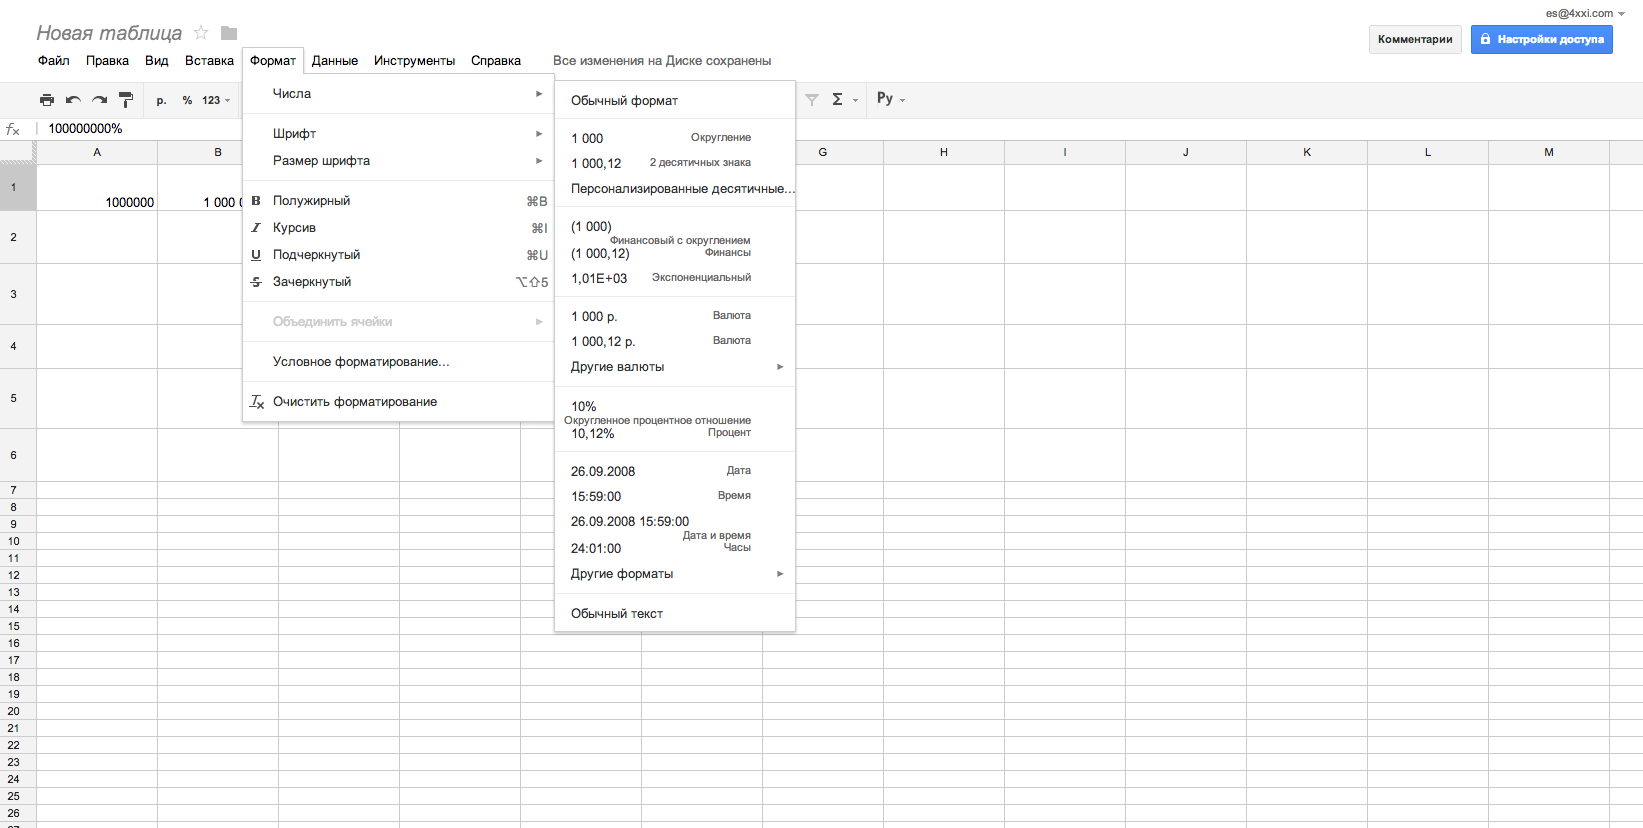
\includegraphics[width=1.0\textwidth]{images/04.png}}
\end{frame}

\section{Формулы}
\subsection{Формулы}
\begin{frame}
  \begin{center}
    \Huge{Формулы}
  \end{center}
\end{frame}

\subsection{Формулы 2}
\begin{frame}[fragile]
  \frametitle{Формулы}
  \begin{itemize}
    \item Формулы --- это то, ради чего используют электронные таблицы.
    \item Формулы позволяют автоматически рассчитывать значения, исходя из данных таблицы.
    \item Пример формулы: =A1+B1.  
    \item Эта формула сложит значения ячеек A1 и B1.
  \end{itemize}
\end{frame}

\subsection{Пример формулы}
\begin{frame}[fragile]
  \frametitle{Пример формулы}
  \centerline{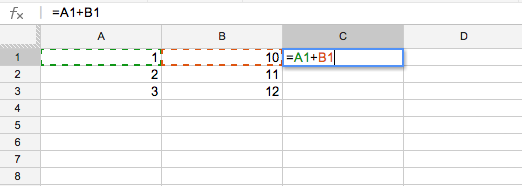
\includegraphics[width=1.0\textwidth]{images/06.png}}
\end{frame}

\subsection{Пример формулы 2}
\begin{frame}[fragile]
  \frametitle{Пример формулы}
  \centerline{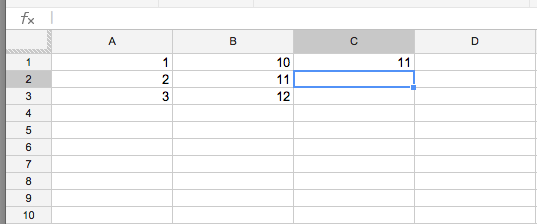
\includegraphics[width=1.0\textwidth]{images/07.png}}
\end{frame}

\subsection{Расширение формул}
\begin{frame}[fragile]
  \frametitle{Расширение формул}
  \centerline{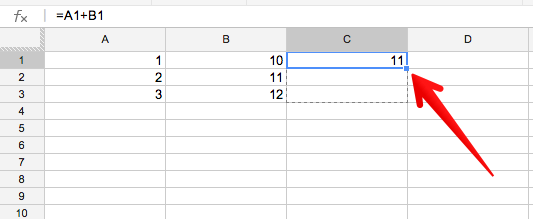
\includegraphics[width=1.0\textwidth]{images/08.png}}
  \begin{itemize}
    \item Если потянуть за маленький квадратик вниз на следующие строки, то \textbf{формулы автоматически скопируются}.
  \end{itemize}
\end{frame}

\subsection{Расширение формул 2}
\begin{frame}[fragile]
  \frametitle{Расширение формул}
  \centerline{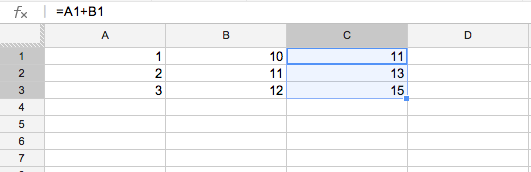
\includegraphics[width=1.0\textwidth]{images/09.png}}
  \begin{itemize}
    \item Таким образом, нам не надо копировать похожие формулы для каждой строки.
  \end{itemize}
\end{frame}

\section{Адресация}
\subsection{Относительная и абсолютная адресации}
\begin{frame}[fragile]
  \frametitle{Относительная и абсолютная адресации}
  \begin{itemize}[<+->]
    \item При копировании формулы изменяются. 
    \item Если вы переносите формулу \textbf{=A1+B1} из ячейки C1 в ячейку C2 (сдвиг на одну строку), то и в формуле всё сдвинется на одну строку:
    \item \textbf{=A2+B2}.
    \item Автоматически, ничего делать не надо, оно само.
    \item При сдвиге на несколько строк (например, из C1 в C3) --- сдвинется на 2.
    \item Абсолютно аналогично со столбцами.
  \end{itemize}
\end{frame}

\subsection{Задачи}
\begin{frame}[fragile]
  \frametitle{Задачи}
  \begin{itemize}[<+->]
    \item Формулу \textbf{=A3+B5} скопировали из ячейки C1 в ячейку C4. Какая формула получилась?
    \item Формулу \textbf{=A3+B5} скопировали из ячейки C1 в ячейку D1. Какая формула получилась?
    \item Формулу \textbf{=A3+B5} скопировали из ячейки C1 в ячейку D3. Какая формула получилась?
    \item Формулу \textbf{=A3+B5} скопировали из ячейки C1 в ячейку F8. Какая формула получилась?
  \end{itemize}
\end{frame}

\subsection{Абсолютная адресация}
\begin{frame}[fragile]
  \frametitle{Абсолютная адресация}
  \centerline{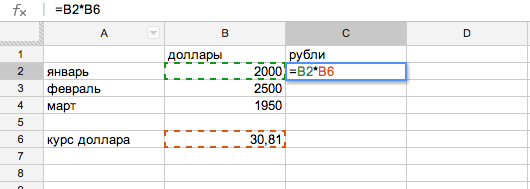
\includegraphics[width=1.0\textwidth]{images/10.png}}
  \begin{itemize}
    \item Но что делать, если я хочу, чтобы какая-то часть формулы не изменялась?
    \item Я хочу, чтобы курс доллара всегда был в ячейке B6.
  \end{itemize}
\end{frame}

\subsection{Абсолютная адресация 2}
\begin{frame}[fragile]
  \frametitle{Абсолютная адресация}
  \centerline{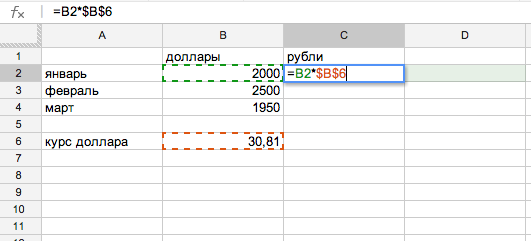
\includegraphics[width=1.0\textwidth]{images/11.png}}
  
  \begin{itemize}
    \item Для этого надо поставить знак доллара перед столбцом (и строкой) в той ячейке, чьё значение мы не хотим изменять.
    \item =B2*\$B\$6.
  \end{itemize}
\end{frame}

\subsection{Задачи}
\begin{frame}[fragile]
  \frametitle{Задачи}
  \begin{itemize}[<+->]
    \item Формулу \textbf{=\$A\$3+B5} скопировали из ячейки C1 в ячейку D4. Какая формула получилась?
    \item Формулу \textbf{=A\$3+B5} скопировали из ячейки C1 в ячейку D4. Какая формула получилась?
    \item Формулу \textbf{=\$A3+B5} скопировали из ячейки C1 в ячейку D4. Какая формула получилась?
    \item Формулу \textbf{=\$A3+B\$5} скопировали из ячейки C1 в ячейку F8. Какая формула получилась?
  \end{itemize}
\end{frame}

\subsection{Задача}
\begin{frame}
  \begin{center}
    \Huge{Депозит}
  \end{center}
  \begin{center}
    \Large{Расчёт прибыли}
  \end{center}
\end{frame}

\subsection{Условие}
\begin{frame}[fragile]
  \frametitle{Условие}
  \begin{itemize}
    \item Допустим, у нас есть 1.000.000 руб.
    \item Мы размещаем депозит в банке под 12 процентов годовых.
    \item Проценты выплачиваются ежемесячно и прибавляются к сумме депозита.
    \item Сколько денег мы будем иметь в конце срока?
  \end{itemize}
\end{frame}

\subsection{Подготовка 1}
\begin{frame}[fragile]
  \frametitle{Подготовка}
  \centerline{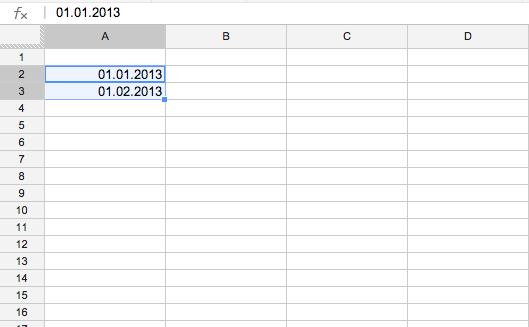
\includegraphics[width=1.0\textwidth]{images/12.png}}
  \begin{itemize}
    \item Напишем первые две даты.
    \item Дальше потянем за синий квадратик. Табличный процессор сам подставит необходимые даты.
  \end{itemize}
\end{frame}

\subsection{Подготовка 2}
\begin{frame}[fragile]
  \frametitle{Подготовка}
  \centerline{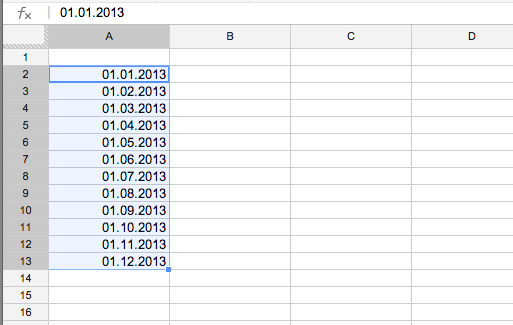
\includegraphics[width=1.0\textwidth]{images/13.png}}
\end{frame}

\subsection{Подготовка 3}
\begin{frame}[fragile]
  \frametitle{Подготовка}
  \centerline{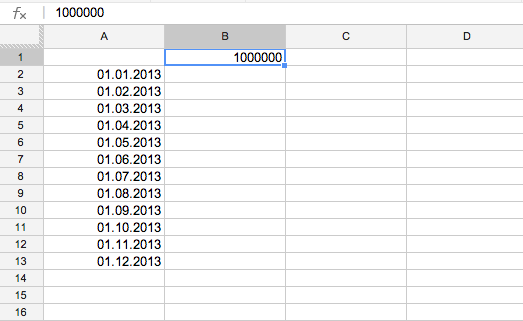
\includegraphics[width=1.0\textwidth]{images/14.png}}
  \begin{itemize}
    \item Укажем исходную сумму в ячейке B1.
  \end{itemize}
\end{frame}

\subsection{Подготовка 4}
\begin{frame}[fragile]
  \frametitle{Подготовка}
  \centerline{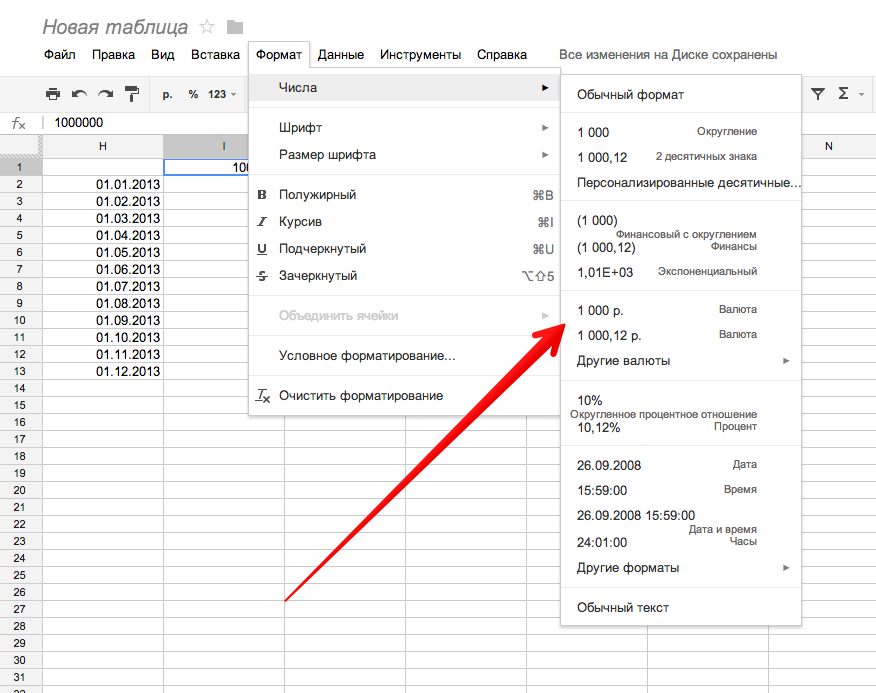
\includegraphics[width=0.7\textwidth]{images/15.png}}
  \begin{itemize}
    \item Преобразуем её в валюту для удобства и красоты.
  \end{itemize}
\end{frame}

\subsection{Работа}
\begin{frame}[fragile]
  \frametitle{Работа}
  \begin{itemize}
    \item Итого, даты есть. В ячейке \textbf{B1} расположена исходная сумма.
    \item Сколько мы получим в первый месяц?
    \item Если за год мы получаем 12\%, то в первый месяц будет: $\cfrac{12}{12} = 1$\%.
    \item Значит, к исходной сумме добавится один процент.
    \item Формула: \textbf{=B1+B1*0.01}.
  \end{itemize}
\end{frame}

\subsection{Работа 2}
\begin{frame}[fragile]
  \frametitle{Работа}
  \centerline{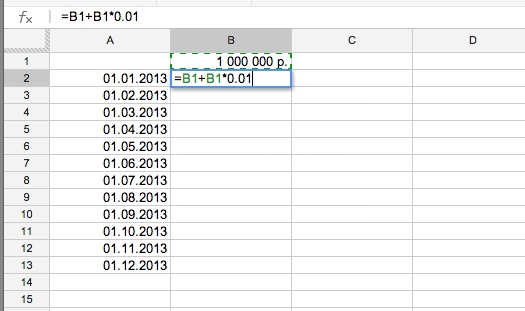
\includegraphics[width=0.8\textwidth]{images/16.png}}
  \begin{itemize}
    \item Введём формулу в соответствующую ячейку.
    \item Скопируем формулу, потянув за синий квадратик. Выделим все числа и преобразуем их в формат валюты.
  \end{itemize}
\end{frame}

\subsection{Результат}
\begin{frame}[fragile]
  \frametitle{Результат}
  \centerline{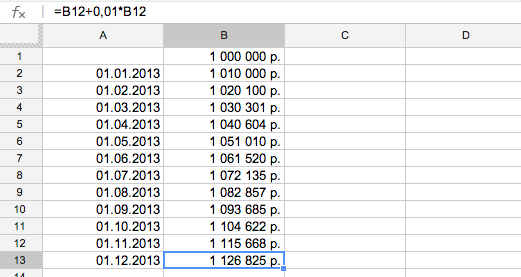
\includegraphics[width=0.8\textwidth]{images/17.png}}
  \begin{itemize}
    \item Итого, получили результат: 1.126.825 руб.
    \item То есть, на 6.825 руб. больше, чем просто 12\% \emph{(сложные проценты)}.
  \end{itemize}
\end{frame}
\end{document}